\documentclass{llncs}
%
%
%espero que no se enfaden por incluir este paquete:
\usepackage{amsmath}
\usepackage[dvips]{graphicx}
\usepackage{makeidx}  % allows for indexgeneration

\hyphenation{pro-per-ties}
\hyphenation{ge-ne-ral-ly}
\hyphenation{pre-fe-ren-ces}
\hyphenation{u-sing}
\hyphenation{pu-nish-ment}

\begin{document}

\mainmatter              % start of the contributions
%
\title{On the cartesian product and the join operations in temporal databases}
%\title{Introducing valid time in bipolar database querying}
%
%\titlerunning{A Fuzzy Valid-Time Model}  % abbreviated title (for running head)
%                                     also used for the TOC unless
%                                     \toctitle is used
%
\author{\and Jose Enrique Pons\inst{1} \and Christophe Billiet\inst{2} \and Guy De Tr\'e\inst{2} \and Olga Pons Capote\inst{1} }

%
%\authorrunning{Ivar Ekeland et al.} % abbreviated author list (for running head)
%
%%%% list of authors for the TOC (use if author list has to be modified)
%\tocauthor{Ivar Ekeland, Roger Temam, Jeffrey Dean, David Grove,
%Craig Chambers, Kim B. Bruce, and Elisa Bertino}
%
\institute{Department of Computer Science and Artificial Intelligence \\
University of Granada \\
C/Periodista Daniel Saucedo Aranda s/n E-18071 (Granada-Spain) \\
\email{jpons,opc@decsai.ugr.es}\\ 
%WWW home page:
%\texttt{http://users/\homedir iekeland/web/welcome.html}
%\and
%Universit\'{e} de Paris-Sud,
%Laboratoire d'Analyse Num\'{e}rique, B\^{a}timent 425,\\
%F-91405 Orsay Cedex, France
\and 
Department of Telecommunications and Information Processing,\\
Ghent University,\\
Sint-Pietersnieuwstraat 41, B-9000 Ghent, Belgium\\
\email{Christophe.Billiet,Guy.DeTre@UGent.be}
}

\maketitle              % typeset the title of the contribution

\begin{abstract}

%%%%%%%%%%%%%%%%%%%%%%%%%
%
% ABSTRACT
%
%%%%%%%%%%%%%%%%%%%%%%%%
In real world, it is very common that some objects or concepts have properties with a time-variant or time-related nature. Modelling this kind of objects or concepts in a (relational) database schema is possible, but time-variant and time-related attributes have an impact on the consistency of the entire database and have to be appropriately managed. Therefore, temporal database models have been proposed to deal with this problem in the literature. Time can be affected by imprecision, vagueness and / or  uncertainty, since existing time measuring devices are inherently imperfect. Additionally, human beings manage time using temporal indications and temporal notions, which may also be imprecise. However, the imperfection in human-used temporal indications is supported by human interpretation, whereas information systems need appropriate support in order to accomplish this task. Several proposals for dealing with such imperfections when modelling temporal data exist. Some of these proposals transform the temporal data into a compact representation but there is not a formal model for managing and handling uncertainty regarding temporal information.
In this work we present a novel model to deal with imprecision in valid-time databases together with the definition and implementation of the data manipulation language, \emph{DML}.


\end{abstract}

%
\section{Introduction}

%
%Information systems (IS) have always tried to model parts of reality. To achieve this modelling, such systems contain data representing properties of real-world objects or concepts~\cite{JoseEnriquePons2012},~\cite{Billiet2012}. As time is an essential aspect of many real-world objects or concepts, information systems often contain data representing temporal notions which describe such temporal properties~\cite{Bolour1982},~\cite{VanderCruyssen1997}. Such temporal notions usually take the form of either instants~\cite{Jensen1998}, which can informally be seen as infinitely short `moments' or `points' in time, or time intervals~\cite{Jensen1998}.

Data are often produced by humans, but human-made data are prone to imperfections: some data may be vague, imprecise, incomplete, contradictory or uncertain. Data representing temporal notions may contain such imprecisions too~\cite{Devos1994},~\cite{Dubois2003},~\cite{JoseEnriquePons2012},~\cite{Billiet2012}. The work presented in this paper is specifically concerned with time intervals (and as a special case: instants) subject to uncertainty.

Generally, one of the most important purposes of an IS is to allow the retrieval of information or knowledge deduced from its data. Information or knowledge is usually retrieved from an IS by querying it and examining or analyzing the query results or by visualizing the contents of the IS, querying this visualization and examining or analyzing the resulting visualization(s).

Of course, when temporal information is represented in an IS, querying this IS may have a temporal aspect too. Usually, querying an IS containing data representing temporal notions is conceptually done by specifying one or more time indications and requesting information that is in a specific relationship with these indications, where the semantics of these relationships are specifically temporal~\cite{Billiet2012},~\cite{JoseEnriquePons2012},~\cite{Pons2012a}. Thus, some existing proposals have considered groups of basic relationships between time indications used to construct and express specific temporal relationships~\cite{Medina1994},~\cite{Schockaert2008}. Notably, Allen~\cite{Allen1983} presented a reasoning framework containing all semantically usefull basic temporal relationships between time intervals (and as a special case instants). The resulting relationships are shown in figure \ref{fig:allen-relationships}. These Allen relationships are used in the presented work.

\begin{figure}[h]
   \centering
   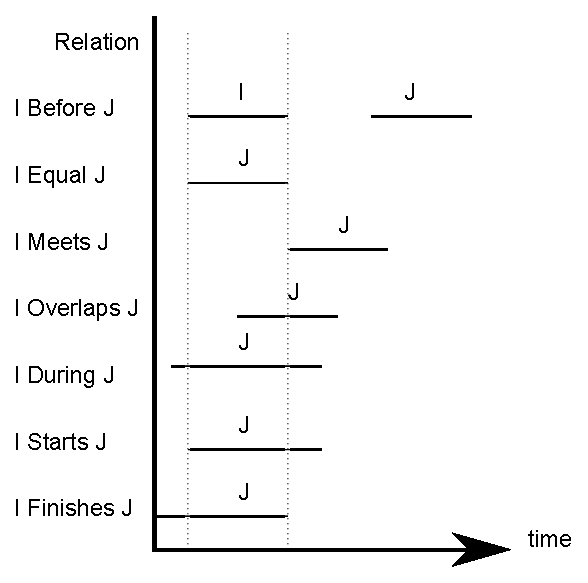
\includegraphics[width=0.9\columnwidth]{graphs/allen.eps}
   \caption{The Allen relationships between two crisp intervals $I$ and $J$.  }
   \label{fig:allen-relationships}
 \end{figure}

To be able to query IS containing data representing time indications subject to uncertainty, a framework is necessary, able to represent uncertainties in time indications in a semantically sound way, without (much) information loss and able to temporally reason with such time indications in a semantically sound and usefull way~\cite{Dubois1983},~\cite{Dubois2003}. Although more proposals for such frameworks exist, the work presented in this paper focusses on just two: the \emph{ill-known constraint \emph{(IKC)} framework}~\cite{Pons2011} and the \emph{triangular model \emph{(TM)} framework}~\cite{DeTre2012}.

The work presented in this paper consists of a comparison of both frameworks, about the approaches they use to represent time intervals subject to uncertainty and to reason about the temporal relationships between such intervals and time intervals without uncertainty.

The structure of this paper is as follows: section \ref{sec:general-preliminaries} presents some general preliminaries and naming and notation conventions used in this paper. Sections \ref{sec:ikc} and \ref{sec:tm} introduce the IKC and TM frameworks respectively: both sections first introduce some preliminary concepts and techniques specific to the framework under consideration, then explain how the representation of time intervals by the framework is done and finally show how the evaluation of Allen relationships between an interval subject to uncertainty and one without uncertainty is done. In section \ref{sec:proposal}, both frameworks are compared: first their approaches to representing time intervals are compared, next their approaches to evaluating Allen relationships are compared. Finally, section \ref{sec:conclusions} presents the principal conclusions of the presented work and some possible future work. 

%TODO: more references in the above part?
%TODO: include some form of proof or previous work with these statements?!

%The concept of the time has been widely studied \cite{Benthem1982}, \cite{Shackle1961}, \cite{Klein1994}. Moreover, humans beings manage temporal indications in an imprecise way \cite{Devos1998}. But when dealing with time in an Information System, some simplifications must to be done. The first thing to do is the discretization of the time line into time points or time intervals. Both approaches have been proved to be equivalent, although due to the nature of the smallest unit of time in a computer, a \emph{chronon}, the discretization of a time point returns a time interval.

%All the possible positions between two time intervals were studied by Allen \cite{Allen1983}, \cite{Allen1985}. As result, the thirteen Allen's Relations were obtained (See Table \ref{tab:allen-relations}) which are illustrated in Figure \ref{fig:allen-relationships}. In order to achieve a more intelligent processing of time, some theoretical frameworks are used to reason with time. First the possibility theory was employed in the reasoning with temporal information \cite{Dubois2003a}. Then, several proposals \cite{Schockaert2008}, \cite{nagypal2003}, \cite{Ohlbach2004}, \cite{Pons2011} studied how to extend the thirteen Allen's relations to the possibilistic case. Also rough set theory \cite{Pawlak1995} has been used to represent and reason about imperfect time intervals \cite{Qiang2009}, \cite{Qiang2010}.

%Although there exists several proposals to represent and visualize imperfect time intervals, in this paper we will focus on two: the ill-known constraint framework \cite{Pons2011} and the triangular model \cite{DeTre2012}. The first one is a theoretical framework that deals with temporal reasoning and the second one is a visual framework that represent imperfect time intervals in a two dimensional space. Both frameworks can be used to represent imperfect time intervals as well as temporal reasoning.

%The structure of this paper is the following. Section  \ref{sec:preliminaries} introduces the Ill-known constraint framework. Section \ref{sec:triangular-model} introduces the triangular model. Section \ref{sec:proposal} analyze both frameworks and shows the correspondences and differences between both frameworks. The section concludes with an example showing that the calculations made in both frameworks are equivalent. Finally, Section \ref{sec:conclusions} presents the main conclusions and the future work. 


%\begin{table}[h]
%\centering
%\begin{tabular}{|c|l|}
%\hline
%Name & Implementation \\ \hline 
%$I$ equals $J$ & if $s_i = s_j \wedge e_i = e_j $ \\
%$I$ starts $J$ & if $s_i = s_j \wedge e_i < e_j $ \\
%$I$ started by $J$ & if $s_i = s_j \wedge e_i > e_j $ \\
%$I$ finishes $J$ & if $s_i > s_j \wedge e_i = e_j $ \\
%$I$ finished by $J$ & if $s_i < s_j \wedge e_i = e_j $ \\
%$I$ meets $J$ & if $e_i = s_j $ \\
%$I$ met by $J$ & if $s_i = e_j $ \\
%$I$ overlaps $J$ & if $s_i < s_j \wedge e_i < e_j \wedge e_i > s_j $ \\
%$I$ overlapped by $J$ & if $s_i > s_j \wedge e_j < e_i \wedge s_i < e_j  $ \\
%$I$ during $J$ & if $s_i > s_j \wedge e_i < e_j $ \\
%$I$ contains $J$ & if $  s_i < s_j \wedge e_i > e_j$ \\
%$I$ before $J$ & if $e_i < s_j $ \\
%$I$ after $J$ & if $s_i > e_j $ \\
%\hline
%\end{tabular}
%\caption{Allen's relations represented in the framework. $I = \left[s_i, e_i\right]$, $J=  \left[s_j, e_j\right]$}
%\label{tab:allen-relations}
%\end{table}



%
\section{\label{sec:prel}Preliminaries}
%

%
%\subsection{\label{sec:bsd}Bipolar Satisfaction Degrees}
%
%\input{bsd}

%
\subsection{Time in databases}
%
%%%%%%%%%%%%%%%%%%%%%%%%%%%%%%%%%%%%%%%%%%%%%%%%%%%%%%%%%%%%%%%%%%%%%%%%%%
%
% Time
%
%%%%%%%%%%%%%%%%%%%%%%%%%%%%%%%%%%%%%%%%%%%%%%%%%%%%%%%%%%%%%%%%%%%%%%%%%
The concept of time has been studied in databases for a long time. A true standard for adding temporal aspects to relational databases does not exist, but there is a consensus in the literature \cite{Dyreson1994} on what is called a \emph{temporal database}: a temporal database is a database dealing with some aspects of time in its schema.
In a temporal DBMS, a \textbf{chronon} is the shortest duration of time supported by the system. In temporal databases, some temporal attributes can be managed without treating the attribute differently from non-temporal attributes. The time described by such an attribute is called \textbf{user defined time} (\emph{UDT}). In addition to UDT, the following types of time can be discerned in a temporal database, all of which are handled exceptionally by the DBMS:

\begin{itemize}
	\item
	\textbf{Transaction time} (\emph{TT}) \cite{L.Rowe1987},\cite{Jensen1991a} denotes the time when the fact (object) is stored in the database. It is usually append-only: as the past can not be changed, TT can not be changed neither. Furthermore, at the moment of insertion, a TT can be neither in the past nor in the future.
	\item
	\textbf{Valid time} (\emph{VT}) \cite{Jensen1994},\cite{Sarda1990} denotes the time when the fact (object) is true in the modelled reality. A fuzzy extension has been proposed by \cite{Garrido2009}. 
%	\item
%	User defined time: It is an uninterpreted attribute. The domain is date/time. The query language has no special support for it.
	\item
	\textbf{Decision time} (\emph{DT}, proposed in \cite{Nascimento1995}) denotes the time when an event was decided to happen. 
	\end{itemize}
	
	E.g., consider a database containing employee contract descriptions. The time when the employee's contract is valid, represented by an interval, is VT. The time when the employee's contract is stored in the database is the TT. The time when the decision for hiring this employee was made is the DT.

% is a non-decomposable unit of time.  it  There are two ways to represent a chronon: as a point or as an interval \cite{655777}.

When working with these time concepts, the Data Manipulation Language (\emph{DML}, which is part of the standard database querying language SQL) is extended to deal with possible temporal inconsistencies within the data and to handle more complex (temporal) queries. 
%Next to these concepts, also \textbf{user defined time} (\emph{UDT}) is discerned. UDT is an uninterpreted attribute in the date/time domain. This means that the attribute uses the date/time domain, but the database model does not treat the attribute differently from non-temporal attributes.
Depending on the time managed, a database is classified as either a \textbf{Valid Time Database} (\emph{VTDB}), a \textbf{Transaction Time Database} (\emph{TTDB}), a \textbf{bi-temporal database} (both valid and transaction time are managed) or a \textbf{tri-temporal database} (valid time, transaction time and decision time are managed).

%\subsection{Temporal Elements}
%%	
%	In order to define a temporal database model, some basic elements should be defined \cite{Dyreson1994}:
%	\begin{itemize}
%	\item A	\textbf{chronon} is a non-decomposable unit of time. In a temporal DBMS, it is the shortest duration of time supported by the system. There are two ways to represent a chronon: as a point or as an interval \cite{655777}.
%	\item
%	\emph{Event}: An instant of time. Usually, an event is said to be occur during time $t$ if it occurs during the chronon represented by $t$.
%	\item
%	\emph{Interval}: The time between two events. The representation is very often a set of contiguous chronons.
	%\item
	%\emph{Span}: A directed duration of time. A duration is an amount of time with known  lenght but no specific starting or ending chronons. The span can be either positive, denoting a forward motion of time or negative, denoting a backward motion of time.
%	\item A	\textbf{timestamp} is a time value associated with some object in the database.	
	
%	\item The	\textbf{lifespan} (of a database object)is the time over which it is defined. The lifespan of a valid time object denotes the time when the corresponding object exists. The lifespan of a transaction time object is the value of the timestamp.
	
	
	
	
	
%	Depending on the type of time the meaning is different:
%		\begin{itemize}
%		\item
%		Lifespan of a valid time object: Refers the time when the corresponding object exists.	
%		\item
%		Lifespan of a transaction time object: The transaction time of a database object refers when the object is stored in the database. The lifespan is the value of the timestamp.		
%		\end{itemize}
%	\end{itemize}
	
%	In the temporal database thesaurus, \emph{'Snapshot'} is the word for non-temporal matters. As a temporal database is a generalization for relational databases, an \emph{snapshot database} is a relational database. Furthermore, a \emph{snapshot relation} is a relation incorporating neither valid nor transaction time.

%\subsection{Main issues when dealing with time}
%Among others, the following problems are present when dealing with time in a database:

%	\begin{itemize}	
%	\item \textbf{Granularity} denotes a partition on the set of chronons. The conversion between several granularities is studied in \cite{Lin97efficientconversion}. Granularity is the base of the temporal model in \cite{Cru97}. An object-oriented implementation is in \cite{624013}.
%	\item	To ensure \textbf{consistency}, temporal databases usually redefine the primary key of a relation. The new primary key takes into account the presence of the time. In order to keep the consistency, the DML is re-defined. For example, in a VTDB, the temporal update sentence is usually composed by an update sentence (closing the old row) plus an insert sentence (creating the new row).
%	\end{itemize}
%Guy's suggestion: instead of imprecision, use imperfection which is more general.
% \subsubsection{Imperfection and time}
% Representing imprecision and its semantics when dealing with time has been studied for a long time. Several proposals for representing and computing imprecise time indications can be found in \cite{DeCaluwe1997} and \cite{DeTre1997a}. Also, the changes between several granularities can be seen as a source of imprecision \cite{Devos1998}.
% 
% In the proposal section we will consider two kinds of imprecision:
% \begin{itemize}
% \item \textbf{Uncertainty in the database} denotes the uncertainty that arises when the knowledge about the temporal data in the database is uncertain. E.g., a database record shows that \emph{`The car is in the garage around April.'}
%  \item \textbf{Imprecision in the query specification} denotes the imprecision in the specification of temporal criteria by the user, when querying. E.g., \emph{`The user wants to obtain a car which is red and which is in the garage around April.'}
% \end{itemize}

\subsubsection{Representation}
Several proposals for managing uncertain time in a database exist. Some proposals work with rough sets \cite{Qiang2009}, other proposals rely on possibility distributions for representing uncertainty in time \cite{Garrido2009}, \cite{Galindo2001}. In order to compare temporal possibility distributions, extensions of the classical Allen's operators \cite{Allen1983} are defined in \cite{Ohlbach2004} and \cite{Nagypal2003}. In the proposal section, we will follow the representation by means of possibility distributions, in order to work with both satisfaction and dissatisfaction degrees. Also, in order to work properly with fuzzy operators, the underlying domain should be numeric. In this paper, the representation for the dates will follow the Julian Day Number (JDN) representation \cite{Husfeld1996}.

If the starting points and/or the end points of the interval representing the time are not known precisely, it is easy to fuzzify them, using, e.g., two triangular possibility distributions.
A \textbf{Fuzzy Validity Period} (\emph{FVP}) is defined as a fuzzy time interval specifying when an object is valid. A fuzzy time interval is then the fuzzification of a crisp time interval. Several options to transform possibility distributions corresponding to the fuzzy starting point and the fuzzy end point into one consistent FVP exist \cite{Garrido2009}, e.g (Fig. \ref{fig:fuzzy-validity-period}):
\begin{itemize}
\item The \textbf{convex hull} approach is the most intuitive approach. The resulting FVP is the convex hull of the union of both fuzzy sets.
\item The \textbf{uncertainty preserving} approach is less intuitive but more realistic. The amount of uncertainty is maintained at the edges of the possibility distribution representing the FVP \cite{Garrido2009}.
\end{itemize}

%%%%%%
% FUZZY VALIDITY PERIOD
%%%%%%
\begin{figure}[h!]
  \centering
  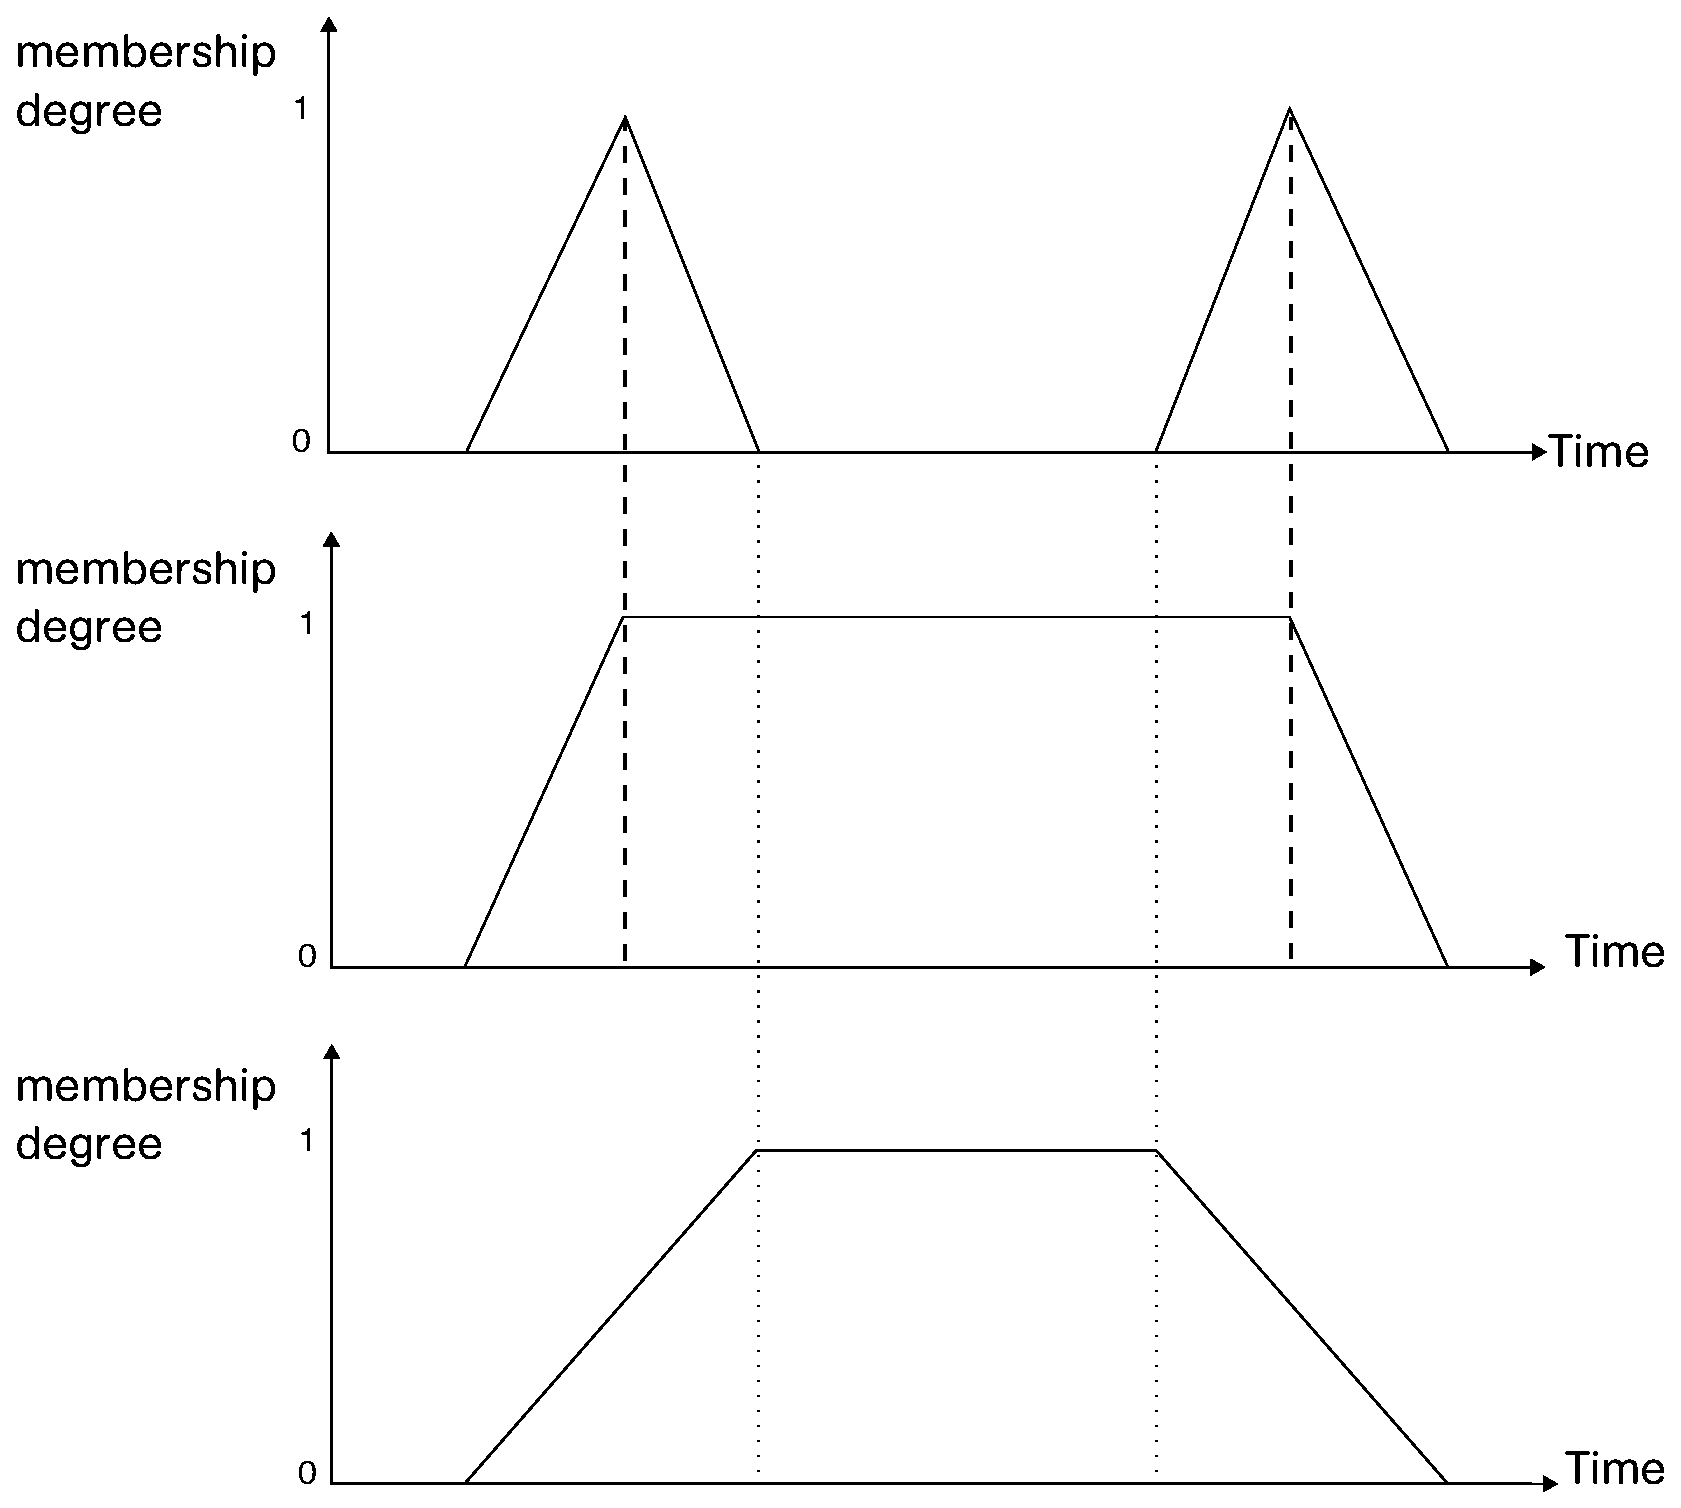
\includegraphics[scale=0.3]{graphs/trapezoidalDistribution.eps}
  \caption{Transformation to obtain the FVP. The top graph shows the two triangular possibility distributions. The middle graph shows the convex hull validity period, the bottom one shows the result of the second transformation, which maintains the imprecision.}
  \label{fig:fuzzy-validity-period}
\end{figure}
%%%%%%%%%%%%%%%%%%%%%%%%%%%%%%
% FVP
%%%%%%%%%%%%%%%%%%%%%%%%%%%%%%%



%
\section{\label{sec:prop}Proposal}
%
%In this section, a valid-time model, able to handle imperfect valid-time notions, will be presented. First, the representation and storage of valid-time will be presented. Next, an approach to query the model is proposed. Finally, an example is given.
%The proposal consist on a possibilistic valid-time model. The representation and the querying are explained in the following subsections.

\subsection{Valid-time Intervals}
\subsubsection{Representation}
\label{subsec:representation-ill-known}
A database models real objects by storing the values of an object for each attribute describing a property of the object. Thus, a valid-time database following the presented proposal will model the time during which an object in a certain state is valid, by associating a \emph{Possibilistic Valid-time Period} (PVP) to the record describing this object state:

\begin{definition}
A \emph{Possibilistic Valid-time Period} is an ill-known interval in time, which models a time period during which an object in a certain state is valid.
\end{definition}

Because a PVP is an ill-known interval, it allows modelling the uncertainty about the start and/or end point of a time interval (and thus about the time interval itself) if such uncertainty exists. The interpretation is \emph{disjunctive}: the PVP represents exactly one valid-time interval, but precisely \emph{which} interval is represented, is (partially) unknown. In the presented model, only PVPs are considered of which the possibility distributions of the possibilistic variables defining the start and end point of the ill-known interval have exactly the same characteristics as the membership functions of fuzzy numbers. A perfectly known start or end point can then be modelled by such an ill-known value defined by a possibilistic variable $P$ for which $\exists ! x : \mu_{P}(x) > 0$.

As mentioned in \cite{Pon11}, this approach differs from the one where a valid-time period is represented by one fuzzy set. Such a fuzzy set is seen as a possibility distribution on $\mathbb{R}$ and thus defines just one ill-known value. However, in the presented approach, a time period is modelled using an ill-known set, which is defined by a possibility distribution on $\Pow(\mathbb{R})$.


%The interval has a starting and an ending points. An ill-known valid-time interval is an interval in witch one or both points are ill-known. 

%\begin{definition}
%A Possibilistic Valid-Time Period \textbf{PVP} is a possibilistic interval defined by means of two ill-known points, namely $\left[ X,\ Y \right]$
%\begin{equation}
%PVP = \left[X,\ Y \right] 
%\end{equation}
%$X$ and $Y$ are ill-known values in the set of the real numbers $\mathbb{R}$. The uncertainty about the values taken by $X$ and $Y$ are given by the possibility distributions $\pi_X$ and $\pi_Y$.
%\end{definition}

%For convenience, the possibility distributions $\pi_X$ and $\pi_Y$ are given in the way of a triangular distribution, as explained in subsection \ref{subsec:fuzzy-numbers}. This representation allows overlapping (Fig. \ref{fig:pvp}). Note that while the two ill-known values $X,Y \in \mathbb{R}$, the fuzzy interval  $[X,Y] \in \mathbb{R}^2$.


%\begin{figure}[h!]
%  \centering
%  %%Created by jPicEdt 1.4.1_03: mixed JPIC-XML/LaTeX format
%%Thu Jun 30 10:32:52 CEST 2011
%%Begin JPIC-XML
%<?xml version="1.0" standalone="yes"?>
%<jpic x-min="5" x-max="125" y-min="5" y-max="65" auto-bounding="true">
%<multicurve fill-style= "none"
%	 points= "(10,10);(10,10);(10,60);(10,60)"
%	 />
%<multicurve fill-style= "none"
%	 points= "(10,10);(10,10);(110,10);(110,10)"
%	 />
%<multicurve fill-style= "none"
%	 points= "(30,10);(30,10);(60,60);(60,60)"
%	 />
%<multicurve fill-style= "none"
%	 stroke-color= "#ccccff"
%	 points= "(60,60);(60,60);(90,10);(90,10)"
%	 />
%<multicurve stroke-width= "0.9"
%	 fill-style= "none"
%	 stroke-color= "#ccccff"
%	 points= "(80,10);(80,10);(100,60);(100,60)"
%	 />
%<multicurve stroke-width= "0.9"
%	 fill-style= "none"
%	 stroke-color= "#ff00cc"
%	 points= "(100,60);(100,60);(110,10);(110,10)"
%	 />
%<text stroke-width= "0.95"
%	 text-vert-align= "center-v"
%	 anchor-point= "(60,65)"
%	 fill-style= "none"
%	 stroke-color= "#ff0033"
%	 text-frame= "noframe"
%	 text-hor-align= "center-h"
%	 >
%X
%</text>
%<text stroke-width= "0.95"
%	 text-vert-align= "center-v"
%	 anchor-point= "(100,65)"
%	 fill-style= "none"
%	 stroke-color= "#ff0033"
%	 text-frame= "noframe"
%	 text-hor-align= "center-h"
%	 >
%Y
%</text>
%<text stroke-width= "0.95"
%	 text-vert-align= "center-v"
%	 anchor-point= "(125,40)"
%	 fill-style= "none"
%	 stroke-color= "#ff0033"
%	 text-frame= "noframe"
%	 text-hor-align= "center-h"
%	 >
%
%</text>
%<text stroke-width= "0.95"
%	 text-vert-align= "center-v"
%	 anchor-point= "(20,5)"
%	 fill-style= "none"
%	 stroke-color= "#ff0033"
%	 text-frame= "noframe"
%	 text-hor-align= "center-h"
%	 >
%1
%</text>
%<text stroke-width= "0.95"
%	 text-vert-align= "center-v"
%	 anchor-point= "(30,5)"
%	 fill-style= "none"
%	 stroke-color= "#ff0033"
%	 text-frame= "noframe"
%	 text-hor-align= "center-h"
%	 >
%2
%</text>
%<text stroke-width= "0.95"
%	 text-vert-align= "center-v"
%	 anchor-point= "(40,5)"
%	 fill-style= "none"
%	 stroke-color= "#ff0033"
%	 text-frame= "noframe"
%	 text-hor-align= "center-h"
%	 >
%3
%</text>
%<text stroke-width= "0.95"
%	 text-vert-align= "center-v"
%	 anchor-point= "(50,5)"
%	 fill-style= "none"
%	 stroke-color= "#ff0033"
%	 text-frame= "noframe"
%	 text-hor-align= "center-h"
%	 >
%4
%</text>
%<text stroke-width= "0.95"
%	 text-vert-align= "center-v"
%	 anchor-point= "(60,5)"
%	 fill-style= "none"
%	 stroke-color= "#ff0033"
%	 text-frame= "noframe"
%	 text-hor-align= "center-h"
%	 >
%5
%</text>
%<text stroke-width= "0.95"
%	 text-vert-align= "center-v"
%	 anchor-point= "(70,5)"
%	 fill-style= "none"
%	 stroke-color= "#ff0033"
%	 text-frame= "noframe"
%	 text-hor-align= "center-h"
%	 >
%6
%</text>
%<text stroke-width= "0.95"
%	 text-vert-align= "center-v"
%	 anchor-point= "(80,5)"
%	 fill-style= "none"
%	 stroke-color= "#ff0033"
%	 text-frame= "noframe"
%	 text-hor-align= "center-h"
%	 >
%7
%</text>
%<text stroke-width= "0.95"
%	 text-vert-align= "center-v"
%	 anchor-point= "(90,5)"
%	 fill-style= "none"
%	 stroke-color= "#ff0033"
%	 text-frame= "noframe"
%	 text-hor-align= "center-h"
%	 >
%8
%</text>
%<text stroke-width= "0.95"
%	 text-vert-align= "center-v"
%	 anchor-point= "(100,5)"
%	 fill-style= "none"
%	 stroke-color= "#ff0033"
%	 text-frame= "noframe"
%	 text-hor-align= "center-h"
%	 >
%9
%</text>
%<text stroke-width= "0.95"
%	 text-vert-align= "center-v"
%	 anchor-point= "(110,5)"
%	 fill-style= "none"
%	 stroke-color= "#ff0033"
%	 text-frame= "noframe"
%	 text-hor-align= "center-h"
%	 >
%10
%</text>
%<text stroke-width= "0.95"
%	 text-vert-align= "center-v"
%	 anchor-point= "(10,5)"
%	 fill-style= "none"
%	 stroke-color= "#ff0033"
%	 text-frame= "noframe"
%	 text-hor-align= "center-h"
%	 >
%0
%</text>
%<text stroke-width= "0.95"
%	 text-vert-align= "center-v"
%	 anchor-point= "(5,60)"
%	 fill-style= "none"
%	 stroke-color= "#ff0033"
%	 text-frame= "noframe"
%	 text-hor-align= "center-h"
%	 >
%1
%</text>
%</jpic>
%%End JPIC-XML
%LaTeX-picture environment using emulated lines and arcs
%You can rescale the whole picture (to 80% for instance) by using the command \def\JPicScale{0.8}
\ifx\JPicScale\undefined\def\JPicScale{1}\fi
\unitlength \JPicScale mm
\begin{picture}(125,65)(0,0)
\linethickness{0.3mm}
\put(10,10){\line(0,1){50}}
\linethickness{0.3mm}
\put(10,10){\line(1,0){100}}
\linethickness{0.3mm}
\multiput(30,10)(0.12,0.2){250}{\line(0,1){0.2}}
\linethickness{0.3mm}
\multiput(60,60)(0.12,-0.2){250}{\line(0,-1){0.2}}
\linethickness{0.9mm}
\multiput(80,10)(0.12,0.3){167}{\line(0,1){0.3}}
\linethickness{0.9mm}
\multiput(100,60)(0.12,-0.6){83}{\line(0,-1){0.6}}
\put(60,65){\makebox(0,0)[cc]{X}}

\put(100,65){\makebox(0,0)[cc]{Y}}

\put(125,40){\makebox(0,0)[cc]{}}

\put(20,5){\makebox(0,0)[cc]{1}}

\put(30,5){\makebox(0,0)[cc]{2}}

\put(40,5){\makebox(0,0)[cc]{3}}

\put(50,5){\makebox(0,0)[cc]{4}}

\put(60,5){\makebox(0,0)[cc]{5}}

\put(70,5){\makebox(0,0)[cc]{6}}

\put(80,5){\makebox(0,0)[cc]{7}}

\put(90,5){\makebox(0,0)[cc]{8}}

\put(100,5){\makebox(0,0)[cc]{9}}

\put(110,5){\makebox(0,0)[cc]{10}}

\put(10,5){\makebox(0,0)[cc]{0}}

\put(5,60){\makebox(0,0)[cc]{1}}

\end{picture}

%  \caption{Two fuzzy numbers $X$ and $Y$ denoting a Possibilistic Valid-Time Period \emph{PVP}.}
%  \label{fig:pvp}
%\end{figure}

\subsubsection{Storage}
\label{subsec:storage}
To store a PVP, the possibility distributions defining the ill-known start and end point are stored. To store such a possibility distribution, the representation as used in the fuzzy interface for relational databases \emph{FIRST}~\cite{Medina94gefred.a}, \cite{Gal98} is used. Using this representation, it is possible to represent not only fuzzy numbers, but also (fuzzy) constants. To store an ill-known value, four values (FT, F1, F2 and F3) are stored. They are explained in Table \ref{table:relational-representation-pvp}. Note that while NULL denotes the fuzzy constant NULL, N denotes a null value in the database \cite{Medina94gefred.a}.

%\begin{itemize}
%\item
%\emph{NULL}: This constant refers to a completely ignorance about the value. The possibility distribution for a given fuzzy number $X$ is not defined, therefore, any comparison between a fuzzy number and the \emph{NULL} constant always returns $0$.
%\item
%\emph{UNKNOWN}: % The possibility distribution for a given fuzzy number $X$ is $\pi_X=1$
%\item
%\emph{UNDEFINED}: The point does not have a value. %The possibility distribution for a given fuzzy number $X$ is $\pi_X=0$
%\end{itemize}
%

\vspace{-10pt}

\begin{table}
\centering
\caption{Relational representation for an ill-known time point. FT denotes Fuzzy Type. Field FT indicates that the values stored in F1, F2 and F3 denote either NULL, UNKNOWN, UNDEFINED or a triangular possibility distribution $M$ = $\left[D,\ a,\ b \right]$. Fields F1, F2 and F3 contain the actual values.}%  A \emph{PVP} is represented by two ill-known points.}
\begin{tabular}{c c c c c c l p{2cm}}
\hline
Value & FT & F1 & F2 & F3 & $\mu(x)$ & Description \\ \hline
UNKNOWN & 0 & N & N & N  & $1$ & Any value is equally possible\\ 
UNDEFINED & 1 & N & N & N & $0$ & The value is not defined \\%in the \\
    %      &   &   &   &   &     & attribute domain\\ 
NULL & 2 & N & N & N &not defined & Nothing is known about the value \\ 
$M$ & 3 & $D$ & $a$ & $b$ & $\mu_{M}$ & Ill-known value \\ 
\hline 
\end{tabular}
\label{table:relational-representation-pvp}

\vspace{10pt}


\end{table}

\vspace{-25pt}

\subsection{Querying Ill-known Valid-time Intervals}
This subsection discusses a tool for querying. Although TSQL~\cite{Jensen1995} is the temporal extension to SQL, the query language proposed is an extension to FSQL~\cite{Gal98} with temporal operators~\cite{Garrido2009}. The focus will evidently lie on the querying of valid-time periods. First, the query structure will be defined, followed by the evaluation and ranking methods.

%In this subsection we will define the query specification, then the evaluation of the query and finally the ranking for the query.

%It is important to notice that every Valid-time notion in the database is represented using a PVP. Thus, Valid-time intervals in the database can be partially unknown.

%In the query, the user is allowed to specify both non-temporal preferences and a temporal constraint.

%This allows the user to specify both the preferences and an ill-known valid-time interval in the query. It is important to notice that the possibilistic / fuzzy data stored in the database has a \emph{disjunctive interpretation} (it is said that we have \emph{uncertainty}: the valid-time interval has only one value but, for some reason the value is ill-known). In the query specification, the user is allowed to express a crisp time interval. 

\subsubsection{Query Structure}
It is important to notice that every valid-time notion in the database is represented using a PVP. In the presented framework, a query has two separate parts:

% one is a temporal constraint and the other is the collection of query specifications for regular attributes:

%the first one is the temporal specification. The second part is the query specification for regular attributes.

\begin{definition}
A query $\tilde Q$ is specified by:
\begin{equation}
\label{eq:query-definition}
\tilde Q = \left( Q^{time}, Q \right)
\end{equation}
\end{definition}
Here, $Q$ denotes the collection of (possibly fuzzy) non-temporal preferences of the user and $Q^{time}$ denotes the temporal constraint given by the user:
\begin{definition}
 $Q^{time}$ is defined by:
\begin{equation}
Q^{time} = \left( I , AR \right)
\end{equation}
\end{definition}
Here, $I$ is a crisp time interval and $AR$ is one of Allen's relations \cite{Allen83}. The interpretation is that for a record with valid-time period given by a PVP $J$, the user requires that $I$ $AR$ $J$ holds.

%In table \ref{tab:allen-relations}, .

%\vspace{-35pt}

\subsubsection{Query evaluation}
In fuzzy querying of regular (relational) databases, the modelling of query satisfaction is a matter of degree. Usually, the evaluation of the query requirements for a record results in a satisfaction degree $s$, where $s$ lies in $\left[0,1\right]$, where 0 denotes total dissatisfaction and 1 denotes complete satisfaction. In crisp querying, the evaluation of query requirements for a record results in the accepting or rejecting of the record as a part of the result set. This can be modelled using satisfaction degrees, by assigning rejection a degree of $0$ and acceptance a degree of $1$ and not using any other value in $\left[0,1\right]$.

The evaluation of a query $\tilde{Q} = \left( Q^{time}, Q \right)$, where $Q^{time} = \left( I, AR \right)$ is now handled as follows. For each record $r$ in the database, with the valid-time notion of $r$ being specified by a PVP $J$, two things happen independently:



% by a combination of non-temporal query requirements $Q$ is noted $e_{Q}(r) \in \left[0,1\right]$ in this work. The total query evaluation method is now the following.  and Allen relation $AR$
\begin{itemize}
\item
The preferences expressed in $Q$ are evaluated, resulting in a satisfaction degree denoted here $e_{Q}(r)$. The presented model accepts any sound way of calculating this evaluation, as long as $e_{Q}(r) \in \left[0,1\right]$. 
\item
Depending on AR, a specific set of ill-known constraints is considered, which can be found in Table 2. The possibility and necessity that $r$ fulfills all these constraints are calculated using formulas based on equations \eqref{ill-known-pos} respectively \eqref{ill-known-nec} and aggregated using the $\min$ operator. 


%The sum of the possibility score and the necessity score gives an evaluation score $e_{Q^{time}}(r)$ in interval $\left[0,2\right]$. Because necessity cannot exceed $0$ unless possibility is $1$, this gives a natural ranking score.
\end{itemize}


\begin{table}[h]
\label{tab:allen-relations}
\caption{Allen's relations used in the framework. Here, $I = \left[a, b\right]$ denotes the PVP in the query, $J = \left[X, Y\right]$ denotes the PVP of the record, with $\pi_{X}$ and $\pi_{Y}$ the possibility distributions of $X$ and $Y$ respectively. For each of Allen's relations $AR$, the corresponding value in column `Constraints' gives the constraints corresponding to $AR$. The last column contains the corresponding formula to calculate the possibility that $I$ satisfies all constraints given in column `Constraints', which are based on equation \eqref{ill-known-pos}.}

\centering
\begin{tabular}{|c|l|l|}
\hline
\multirow{2}{*}
{Allen Relation}  & {Constraints} & $\Pos($ I satisfies all constraints  \\
 & & $C_{i}, i = 1,2,\ldots)$ \\
\hline
I before J & $C_1 \triangleq \left(<,X\right)$ & $\sup_{a>w}\pi_x(w)$\\
\hline

\multirow{2}{*}
{I equal J} & $C_1\triangleq \left(\geq,X\right)$,$C_2\triangleq \left(\neq,X\right)$ & $\min ( \sup_{a \leq w}\pi_x(w),\pi_x(w),$ \\
 & $C_3\triangleq \left(\leq,Y\right)$,$C_4\triangleq \left(\neq,Y\right)$ & $\sup_{b \geq w}\pi_Y(w),\pi_Y(w))$\\
\hline

I meets J & $C_1\triangleq \left(\leq,X\right)$ ,$C_2\triangleq \left(\neq,X\right)$ & $\min (\sup_{a\geq w} \pi_X(w),$ $\pi_X(w))$ \\
\hline

\multirow{2}{*}
{I overlaps J} & $C_1\triangleq \left(<,Y\right)$,$C_2\triangleq \left(\leq,X\right)$ & $\min ( \sup_{b>w}\pi_Y(w), $ \\
 & $C_3\triangleq \left(\geq,X\right)$ & $\sup_{a \geq w}\pi_X(w),\sup_{a \leq w}\pi_X(w))$ \\
\hline

\multirow{2}{*}
{I during J} & $C_1\triangleq \left(>,X\right)$, $C_2\triangleq \left(\leq,Y\right)$ & $\max ( \min ( \sup_{a<w}\pi_X(w),\sup_{b \geq w}\pi_Y(w)),$ \\
 & $C_3\triangleq \left(\geq,X\right)$ ,$C_4\triangleq \left(<,Y\right)$ & $\min ( \sup_{a \leq w }\pi_X(w),\sup_{b>w}\pi_Y(w)$\\
\hline

{I starts J} & $C_1\triangleq \left(\geq,X\right)$,$C_2\triangleq \left(\neq,X\right)$  & $\min( \sup_{a \leq w}\pi_X(w),$ $\pi_X(w))$\\
\hline

{I finishes J} & $C_1\triangleq \left(\leq,Y\right)$, $C_2\triangleq \left(\neq,Y\right)$  & $\min ( \sup_{b \geq w} \pi_Y(w),$ $\pi_Y(w))$ \\
\hline 

\end{tabular}

\vspace{10pt}


\vspace{-25pt}

\end{table}


\vspace{-5pt}

\subsubsection{Ranking and aggregation}
In order to present the results to the user, a crude ranking method is used: for every record $r$, the sum of $\Pos_{Q^{time}}(r)$ and $\Nec_{Q^{time}}(r)$ gives an evaluation score $e'_{Q^{time}}(r)$ in interval $\left[0,2\right]$. Because necessity cannot exceed $0$ unless possibility is $1$, this gives a natural ranking score. Some authors ~\cite{Bosc2010a} mentioned before that the possibility and necessity measures result in a total order in the set of events.  This $e'_{Q^{time}}(r)$ is then rescaled to the unit interval, resulting in $e_{Q^{time}}(r)$. The final ranking $e_{final}(r)$ is now given by a convex combination:

%the possibility and the necessity are ranked with the convex combination in \eqref{eq:convex-comb} with $\omega=0.5$. Finally this value is aggregated with the rest of the criteria with the same combination. %In this case the value for the aggregation is also $\omega = 0.5$

\begin{equation}
\label{eq:convex-comb}
e_{final}(r)\ =\ \omega*e_{Q}(r)\ +\ (1-\omega)*e_{Q^{time}}(r), \omega \in \left[0, 1 \right]
\end{equation}

The use of this convex combination allows a record to make up for a low score for the temporal constraint by a good score for the non-temporal constraint (or vice versa). Changing $\omega$ also allows granting the temporal constraint more weight with respect to the non-temporal constraint (or vice versa).

%By increasing the value for the parameter $\omega$, the preferences expressed in the query $Q$ can be given more importance. By lowering the value for $\omega$, the temporal criteria is emphasized.
%The following example illustrates the querying process.

%\subsection{Example}

\begin{example} 

%\subsubsection{The database}
%\paragraph{The database}
Consider the example relation given in Table \ref{tb:car-models} describing car models, containing general attributes (model name, manufacturer, car segment) and one temporal attribute (stored as explained in subsection \ref{subsec:storage}) describing the approximate period of time during which the car model was sold. The value for $D$ is stored in \emph{yyyy} format and $a$ and $b$ are represented by an integer. The ID field identifies a car model while the field Instance ID (IID) identifies the instance for a car model, thus a car model in a certain state.

\end{example}
%%%%%%%%%%%%%%%%%%%%%%%%%%%%%%%%%%%%%%%%%%%%%%%%%%
% Sample table for the car models. 
%%%%%%%%%%%%%%%%%%%%%%%%%%%%%%%%%%%%%%%%%%%%%%%%%%%
\begin{table}[h]
\centering
\caption{Example database}
\begin{tabular}{c c c c c c c}
\hline
ID & IID & Segment & Manufacturer & Name & Start & End  \\ [0.5ex]
\hline
001 & 1 & B & Peugeot & 205 & [1985,2,3] & [1997,2,1] \\
002 & 1 & C & Peugeot & 305 & [1977,2,2] & [1989,2,3] \\
003 & 1 & B & Citroen & C2 & [2002,2,2] & [2006,1,1] \\
001 & 2 & B & Peugeot & 206 & [2000,1,2] & [2011,2,1] \\
001 & 3 & B & Peugeot & 207 & [2006,1,1] & [2011,1,1]\\
\hline
\end{tabular}
\vspace{10pt}
\label{tb:car-models}
\vspace{-30pt}
\end{table}

%\subsubsection{The query}
%\paragraph{The query}
Consider the following query:
\begin{center}
\emph{The user wants to obtain a list of models from segment B, made by manufacturer Peugeot before the year interval 2001-2005}\\
\end{center}

Using the introduced notations in \eqref{eq:query-definition}, the query is translated to: %the following expression:

%\vspace{-10pt}
%
%\begin{align}
%$\tilde{Q} = \left(Q^{time}, Q\right)$
%\end{center}
%
%\vspace{-10pt}
%
%In this expression:
%\begin{itemize}
%\item
%$Q^{time}\ = \ ( \left[ 2001,\ 2005 \right],\ $  before $)$.
%\item
%$c_{segment}\ = \ $ Peugeot.
%\end{itemize}

%\vspace{-15pt}

\begin{align}
Q^{time} & = \left(\left[ 2001, 2005 \right], before\right) \\
Q & = \left(Segment =  B\right) \wedge \left(Manufacturer = Peugeot\right)
\end{align}

%The evaluation for the criteria are presented in the result table \ref{tb:results}.

\begin{table}[ht]
\caption{Result table and ranking}
\centering
\begin{tabular}{c c c c c c c}
\hline
ID & IID &  $\Pos_{Q^{time}}$ & $\Nec_{Q^{time}}$ & $e_{Q^{time}} (rescaled)$ & $Q$ & $e_{final}$ ($\omega=0.5$) \\ [0.5ex]
\hline
001 & 1 & 1 &  1 & 1 & 1 & 1 \\
002 & 1 & 1 & 1 & 1 & 0.5 & 0.75 \\
003 & 1 & 1 & 0.5 & 0.75 &0 & 0.375\\
001 & 2 & 1 & 0 & 0.5 &1 & 0.75 \\
001 & 3 & 0 & 0 & 0 &1 & 0.5\\
\hline
\end{tabular}
\label{tb:results}
\end{table}


Table \ref{tb:results} shows a natural and gradual ranking for the results. The last record, (ID 001, IID 3) shows also that with $\omega$ = 0.5 both temporal and regular criteria have the same importance.% By lowering the value for omega the temporal criteria would have more impact on the final ranking.




%
\section{\label{sec:conc}Conclusions}
%
%In this paper, a comparison is presented between two different frameworks designed to represent time intervals subject to uncertainty and evaluate temporal relationships between such intervals and crisp intervals: the triangular model (TM) framework and the ill-known constraint (IKC) framework. It is concluded that:

\begin{itemize}
	\item With respect to representation, both frameworks differ only slightly, with the TM framework allowing easier human assessments, due to its approach including visualization.
	\item With respect to temporal relationship evaluation, the TM framework allows easy human assessments in several situations, but the IKC framework seems more fitted for complex reasoning, due to its modular build.
\end{itemize}

Future research will deal with the evaluation of temporal relationships between several time intervals subject to uncertainty and with querying aspects in both frameworks.
%
\subsubsection{Acknowledgements}
%
%%%%%%%%%%%%%%%%%%%%%%%%%%%%%%%%%%%%%%%%%%%%%%%%%%%%%%%%%%%%%%%%%%%%%%%%%
%
% Acknowledgements
%
%%%%%%%%%%%%%%%%%%%%%%%%%%%%%%%%%%%%%%%%%%%%%%%%%%%%%%%%%%%%%%%%%%%%%%%%%
Part of the research is supported by the grant BES-2009-013805 within the research project TIN2008-02066: \emph{Fuzzy Temporal Information treatment in relational DBMS}.



\bibliographystyle{splncs03}
\bibliography{fqas}




\end{document}


